
\documentclass{article}

\setlength{\oddsidemargin}{0.05 in}
\setlength{\evensidemargin}{-0.05 in}
\setlength{\topmargin}{-0.6 in}
\setlength{\textwidth}{6.5 in}
\setlength{\textheight}{9.5 in}
\setlength{\headsep}{0.25 in}
\setlength{\parskip}{0.1 in}

%
% ADD PACKAGES here:
\usepackage [usenames] {color}
\definecolor {infocolor} {rgb} {0.6,0.6,0.6}
\definecolor {steel blue}{rgb}{0.274510,0.509804,0.705882}
\everymath{\color{steel blue}}
\everydisplay{\color{steel blue}}
%
\usepackage{tikz}
\usetikzlibrary{calc}

\usepackage{amsmath,amsfonts,amssymb,enumerate,graphicx}

%
% The following commands set up the lecnum (lecture number)
% counter and make various numbering schemes work relative
% to the lecture number.
%
\newcounter{lecnum}
\renewcommand{\thepage}{\thelecnum-\arabic{page}}
\renewcommand{\thesection}{\thelecnum.\arabic{section}}
\renewcommand{\theequation}{\thelecnum.\arabic{equation}}
\renewcommand{\thefigure}{\thelecnum.\arabic{figure}}
\renewcommand{\thetable}{\thelecnum.\arabic{table}}

\DeclareMathOperator{\rk}{rk}

\newcommand{\tran}{^{\mbox{\tiny $\top$}}}
\newcommand{\tleq}{^{\mbox{\tiny $\leqslant$}}}
\newcommand{\teq}{^{\mbox{\tiny $=$}}}

%
% The following macro is used to generate the header.
%
\newcommand{\lecture}[2]{
   \pagestyle{myheadings}
   \thispagestyle{plain}
   \newpage
   \setcounter{lecnum}{#1}
   \setcounter{page}{1}
   \noindent
   \begin{center}
       \vbox{\vspace{2mm}
         \hbox {\leftline{\Large LECTURE #1: \hfill}}
         \vspace{3mm}
         \hbox {\leftline{\Large #2 \hfill}}
         \vspace{4mm}
         \hrule
         \vspace{3mm}
         \hbox to 6.5in { {{\large Polyhedral Theory}  \hfill April 2013} }
         \vspace{3mm}
        }
   \end{center}
   \markboth{LECTURE #1: #2}{LECTURE #1: #2}
   \pagenumbering{arabic}
   \vspace*{4mm}
}
%
% Convention for citations is authors' initials followed by the year.
% For example, to cite a paper by Leighton and Maggs you would type
% \cite{LM89}, and to cite a paper by Strassen you would type \cite{S69}.
% (To avoid bibliography problems, for now we redefine the \cite command.)
% Also commands that create a suitable format for the reference list.
\renewcommand{\cite}[1]{[#1]}
\def\beginrefs{\begin{list}%
        {[\arabic{equation}]}{\usecounter{equation}
         \setlength{\leftmargin}{2.0truecm}\setlength{\labelsep}{0.4truecm}%
         \setlength{\labelwidth}{1.6truecm}}}
\def\endrefs{\end{list}}
\def\bibentry#1{\item[\hbox{[#1]}]}

%Use this command for a figure; it puts a figure in wherever you want it.
%usage: \fig{NUMBER}{SPACE-IN-INCHES}{CAPTION}
\newcommand{\fig}[3]{
            \vspace{#2}
        	\begin{center}
			Figure \thelecnum.#1:~#3
			\end{center}
	}
% Use these for theorems, lemmas, proofs, etc.
\newtheorem{theorem}{Theorem}[lecnum]
\newtheorem{lemma}[theorem]{Lemma}
\newtheorem{proposition}[theorem]{Proposition}
\newtheorem{claim}[theorem]{Claim}
\newtheorem{corollary}[theorem]{Corollary}
\newtheorem{definition}[theorem]{Definition}
\newenvironment{proof}{{\it Proof.}}{ \hfill $\square$}

% **** IF YOU WANT TO DEFINE ADDITIONAL MACROS FOR YOURSELF, PUT THEM HERE:

\def\R{{\mathbb R}}
\def\Q{{\mathbb Q}}
\def\Z{{\mathbb Z}}
\def\K{{\mathbb K}}

\begin{document}
%FILL IN THE RIGHT INFO.
%\lecture{**LECTURE-NUMBER**}{**DATE**}{**LECTURER**}{**SCRIBE**}
\lecture{6}{Integer polyhedra}
%\footnotetext{These notes are partially based on those of Nigel Mansell.}

% **** YOUR NOTES GO HERE:

% Some general latex examples and examples making use of the
% macros follow.
%**** IN GENERAL, BE BRIEF. LONG SCRIBE NOTES, NO MATTER HOW WELL WRITTEN,
%**** ARE NEVER READ BY ANYBODY.

\section{Hilbert basis}
The Hermite normal form $[B~\boldsymbol{0}]$ of a rational matrix $A\in \Q^{m\times n}$ can be considered as a minimal generating set of the lattice $\Lambda(A)$ generated by $A$.

In this section, we are going to deal with the lattice points in a polyhedral cone. Is there any similar basis for the integer points in a polyhedral cone $C$ generated by rational vectors $\{a_1,\dots,a_n\}$? A finite set of vectors $\{a_1,\dots,a_t\}$ is a \emph{\textbf{Hilbert basis}} if each integral vector $b$ in $\mbox{cone}\{a_1,\dots,a_t\}$ is a non-negative integral combination of $a_1,\dots,a_t$. Especially, we are interested in \emph{\textbf{integral Hilbert bases}}, which are Hilbert bases consisting of integral vectors only. 

\begin{theorem}
Each rational polyhedral cone $C$ is generated by an integral Hilbert basis. Furthermore, if $C$ is pointed, the minimal integral Hilbert basis is unique (minimal relative to set inclusion).
\end{theorem}
\begin{proof}
Without loss of generality, let $C$ be generated by integral vectors $a_1,\dots,a_s$, i.e., $C=\mbox{cone}\{a_1,\dots,a_s\}$. We claim that the finite set $H=\{h_1,\dots,h_t\}$ of integral vectors contained in the zonotope
$$Z:=\{x\in\R^n~|~x=\sum_{i=1}^t \lambda_i a_i, 0\leqslant\lambda_i\leqslant 1~\mbox{for}~i=1,\dots,t\}$$
is a Hilbert basis. Following is an example with $n=2$, $s=2$ and $t=8$.

\begin{figure}[h!]
  \centering
    \begin{tikzpicture}
      \draw[thick] (-0.5,0) -- (4.5,0);
      \draw[thick] (0,-0.5) -- (0,4.5);
      \draw[thin] (0,0) -- (2,4);
      \draw[thin] (0,0) -- (4,1.3333333333);
      
      \draw[thin,-latex,dashed, fill=gray, fill opacity=0.3] (0,0) -- (0.5,1) --
        (2,1.5) -- (1.5,0.5) -- cycle;
      
      \draw[thick,-latex,] (0,0) -- (0.5,1) node [above left] {$a_1$};
      \draw[thick,-latex,] (0,0) -- (1.5,0.5) node [below right] {$a_2$}; 
      
      \foreach \x in {0,1,...,8} 
        \foreach \y in {0,1,...,8} 
          \node[draw,step=0.5cm,circle,inner sep=0.8pt,fill] at (0.5*\x,0.5*\y) {}; % Places a dot at those points
          %\draw[help lines,fill] (\x,\y)  circle (1pt);

       \draw[ultra thick,red] (0.95,0.45) node [above] {$Z$}; 
       \draw[ultra thick,red] (2.4,1.9) node [above right] {\Large $C$}; 
       
        \node[draw=red, shape=circle, inner sep=1pt, fill=red] at (0,0){}; 
        \node[draw=red, shape=circle, inner sep=1pt, fill=red] at (0.5,0.5){}; 
        \node[draw=red, shape=circle, inner sep=1pt, fill=red] at (0.5,1){}; 
        \node[draw=red, shape=circle, inner sep=1pt, fill=red] at (1,0.5){}; 
        \node[draw=red, shape=circle, inner sep=1pt, fill=red] at (1,1){}; 
        \node[draw=red, shape=circle, inner sep=1pt, fill=red] at (1.5,0.5){}; 
        \node[draw=red, shape=circle, inner sep=1pt, fill=red] at (1.5,1){}; 
        \node[draw=red, shape=circle, inner sep=1pt, fill=red] at (2,1.5){}; 
    \end{tikzpicture}
  \caption{The cone $C$ and the polytope $Z$}
\end{figure}

Clearly, $H$ generates $C$, as $a_1,\dots,a_s$ are contained in $H$. To see that vectors in $H$ form a Hilbert basis, let $p\in C\cap\Z^n$. Then, we have
$$
p=\sum_{i=1}^s \lambda_i a_i, \lambda_i\geqslant 0,i=1,\dots,t,
$$
for some $\lambda_i$ (not necessarily integer). Furthermore, we have
$$
p-\sum_{i=1}^s \lfloor\lambda_i\rfloor a_i=\sum_{i=1}^s(\lambda_i-\lfloor\lambda_i\rfloor)a_i.
$$
Then the RHS vector above occurs in $H$, as the LHS is integral, and the RHS belongs to $Z$. Since $a_1,\dots,a_s$ are also contained in $H$, it follows that (16) decompose $p$ into a non-negative integral combination of $H$. So vectors in $H$ form a Hilbert basis.

Next, suppose $C$ is pointed.

\end{proof}




\section{Integer hulls and integer polyhedra}
The \emph{\textbf{integer hull}} $P_I$ of $P$ is defined by:
\begin{equation}
P_I:=\mbox{conv}(P\cap \Z^n).
\end{equation}
So the integer hull $P_I$ of $P$ is the convex hull of the integral vectors in $P$. A rational polyhedron $P$ is an \emph{\textbf{integer polyhedron}} if $P=P_I$. Clearly, for any rational polyhedral cone $C$, $C=C_I$, as $C$ is generated by rational, and hence integral, vectors. Therefore, a rational polyhedral cone is always an integer polyhedron.

\begin{theorem}
The integer hull $P_I$ of a rational polyhedron $P$ is a polyhedron. If $P_I\not=\emptyset$, then $\mbox{rec}(P)=\mbox{rec}(P_I)$.
\end{theorem}
\begin{proof}
(1) If $P$ is a polytope(thus bounded), then $\lvert P\cap\Z^n \rvert$ is finite, so $P_I$ is a polytope.\\
(2) If $P$ is a polyhedral cone, then $P=P_I$.\\
(3) Assume $P=Q+C$, where $Q$ is polytope and $C$ is the characteristic cone of $P$. Let $C$ be generated by $a_1,\dots,a_s\in \Z^n$ and let $Z$ be the polytope (parallelepiped, strictly speaking zonotope)
\begin{equation}
Z:=\{\sum_{i=1}^{s} \lambda_i a_i~|~0\leqslant \lambda_i\leqslant 1~\mbox{for}~i=1,\dots,s\}.
\end{equation}
We show that 
\begin{equation}
P_I=(Q+Z)_I+C,
\end{equation} which implies the theorem, as $Q+Z$ is a polytope, and hence $(Q+Z)_I$ is a polytope.

\begin{figure}[h!]
  \centering
    \begin{tikzpicture}
      \draw[thick] (-0.5,0) -- (4.5,0);
      \draw[thick] (0,-0.5) -- (0,4.5);
      \draw[thin] (0,0) -- (0.5,1);
      \draw[thin, dashed] (0.5,1) -- (2,4);
      \draw[thin] (0,0) -- (1.5,0.5);
      \draw[thin, dashed] (1.5,0.5) -- (4, 1.333333333333);
      \draw[thick] (1.25,0.916666666667) -- (4.5, 2);
      \draw[thick] (0.9,2.85) -- (1.8, 4.6);
      \draw[thin] (1.25,0.916666666667) -- (0.9,2.85);
      \draw[thick] (0.65,1.75) -- (0.9,2.85);
      \draw[thick] (0.65,1.75) -- (1.25,0.916666666667);
      \draw[thin, -latex] (1.25,0.916666666667) -- (1.25+0.5,0.916666666667+1);
      \draw[thin, -latex] (1.25,0.916666666667) -- (1.25+1.5,0.916666666667+0.5);
      \draw[thin, dashed] (1.25+0.5,0.916666666667+1) -- (1.25+0.5+1.5,0.916666666667+1+0.5);
      \draw[thick] (1.25+0.5+1.5,0.916666666667+1+0.5) -- (1.25+0.5+1.5-0.5,0.916666666667+1+0.5-1);
      \draw[thin, -latex] (0.65,1.75) -- (0.65+0.5,1.75+1);
      \draw[thin, -latex] (0.65,1.75) -- (0.65+1.5,1.75+0.5);
      \draw[thin, dashed] (0.65+0.5,1.75+1) -- (0.65+0.5+1.5,1.75+1+0.5);
      \draw[thin, dashed] (0.65+1.5,1.75+0.5) -- (0.65+0.5+1.5,1.75+1+0.5);
      \draw[thin, -latex] (0.9,2.85) -- (0.9+1.5,2.85+0.5);
      \draw[thin, -latex] (0.9,2.85) -- (0.9+0.5,2.85+1);
      \draw[thin, dashed] (0.9+1.5,2.85+0.5) -- (0.9+1.5+0.5,2.85+0.5+1);
      \draw[thick] (0.9+1.5+0.5,2.85+0.5+1) -- (0.9+1.5+0.5-1.5,2.85+0.5+1-0.5);
      
      \draw[thick] (0.9+1.5+0.5,2.85+0.5+1) -- (1.25+0.5+1.5,0.916666666667+1+0.5);
      
      \draw[thin,-latex,dashed, fill=gray, fill opacity=0.3] (0,0) -- (0.5,1) --
        (2,1.5) -- (1.5,0.5) -- cycle;
      
      \draw[thin,-latex,dashed, fill=gray, fill opacity=0.3] (0.65,1.75) -- (0.9,2.85)   
        --(1.25,0.916666667) -- cycle;
      
      \draw[thin,-latex] (0,0) -- (0.5,1) node [above left] {$a_1$};
      \draw[thin,-latex] (0,0) -- (1.5,0.5) node [below right] {$a_2$}; 
      
      \node[draw, shape=circle, inner sep=1pt] at (1.25,0.916666666667){};
      \node[draw, shape=circle, inner sep=1pt] at (0.65,1.75){};
      \node[draw, shape=circle, inner sep=1pt] at (0.9,2.85){}; 
      
      \foreach \x in {0,1,...,8} 
        \foreach \y in {0,1,...,8} 
          \node[draw,step=0.5cm,circle,inner sep=0.85pt,fill] at (0.5*\x,0.5*\y) {}; % Places a dot at those points
          %\draw[help lines,fill] (\x,\y)  circle (1pt);

      \foreach \y in {3,4,5,6}
        \node[draw=red, fill=red, shape=circle, inner sep=1pt] at (1,0.5*\y) {};

      \foreach \y in {2,3,4,5,6,7}
        \node[draw=red, fill=red, shape=circle, inner sep=1pt] at (1.5,0.5*\y) {};

      \foreach \y in {3,4,5,6,7,8}
        \node[draw=red, fill=red, shape=circle, inner sep=1pt] at (2,0.5*\y) {};

      \foreach \y in {3,4,5,6,7,8}
        \node[draw=red, fill=red, shape=circle, inner sep=1pt] at (2.5,0.5*\y) {};
        
      \foreach \y in {4,5,6,7}
        \node[draw=red, fill=red, shape=circle, inner sep=1pt] at (3,0.5*\y) {};
        
      \draw[thin,red,-latex,fill opacity=0.3] (1.5,1) -- (2.5,1.5) -- (3,2) -- (3,3.5)
        --(2.5,4) -- (2,4) -- (1,3) -- (1,1.5) -- cycle;
    
       \draw[ultra thick,red] (0.95,0.45) node [above] {$Z$}; 
       \draw[ultra thick,red] (0.87,1.46) node [above] {$Q$}; 
       \draw[ultra thick,red] (2,2.4) node [above] {\large $Q+Z$}; 
       \draw[ultra thick,red] (2.4,1.9) node [above right] {\Large $C$}; 
    \end{tikzpicture}
  \caption{The structure of integer hull}
\end{figure}

To see $(Q+Z)_I+C\subseteq P_I$, observe
\begin{equation}
(Q+Z)_I+C\subseteq P_I+C=P_I+C_I\subseteq (P+C)_I=P_I.
\end{equation}
The first inclusion comes from the fact that $Q+Z\subseteq P$. Since each integral vector in $Q+Z$ is also a integral vector in $P$, therefore $(Q+Z)_I\subseteq P_I$. As to the second inclusion, since the sum of any two integral vectors from $P$ and $C$ is still a integral vector in $P+C$, i.e., $(P\cap \Z^n)+(C\cap \Z^n) \subseteq (P+C)\cap \Z^n$, together with the property of Minkowski sum $P_I + C_I=\mbox{conv}\{P\cap \Z^n + C\cap \Z^n\}$, the second inclusion follows.

For the reverse inclusion, let $p\in P\cap\Z^n$. Then $p=q+c$ for some $q\in Q$ and $c\in C$. Note that $c=\sum_i \lambda_i a_i=\sum_i\left\lfloor \lambda_i \right\rfloor  a_i+\sum_I(\lambda_i-\left\lfloor \lambda_i \right\rfloor)a_i$, where the first term is denoted by $c^\prime$ and the second by $z$. Clearly, $c^\prime \in C\cap \Z^n$ and $z\in Z$. It follows that $p=(q+z)+c^\prime$ and $q+z\in (Q+Z)_I$(as $q+z=p-c^\prime$ and $p$ and $c^\prime$ are integral). Since $c^\prime\in C$, we have $p\in (Q+Z)_I+C$.

If $P_I\not=\emptyset$, then the characteristic cone of $P_I$ is uniquely defined by the decomposition in (6.3). Hence, $\mbox{rec}(P)=C=\mbox{rec}(P_I)$.
\end{proof}

So in principle, an ILP is just a LP over the integer hull of a polyhedron.


\begin{proposition}
Let $P$ be a rational polyhedron. Then the following  are equivalent.
\begin{enumerate}
\item[(1)] $P=P_I$, i.e., $P$ is the convex hull of the integral vectors in $P$,
\item[(2)] each face of $P$ contains integral points,
\item[(3)] each minimal face of $P$ contains integral points,
\item[(4)] $\max\{c^T x~|~x\in P\}$ is attained by a integral point, for each $c\in\R^b$ for which the maximum is finite.
\end{enumerate}
\end{proposition}
\begin{proof}
\end{proof}


So in particular, if $P$ is pointed, then $P=P_I$ if and only if each vertex of $P$ is integral.

\section{Unimodular transformations and integer polyhedra}
Recall that affine images of polyhedra are polyhedra. Clearly the same is true for rational polyhedra and rational affine maps (i.e., affine maps $x\rightarrow Mx+t$ for a rational matrix $M\in\Q^{m\times n}$ and a rational vector $t\in \Q^n$). In the previous notes, we have sometimes used affine transformations to obtain a nice representation of polyhedra. For example, up to an affine map we can assume that a polyhedron is full-dimensional. Another example is the Gaussian elimination method. Implicitly, we perform affine transformation when we solve systems using Gaussian elimination. All row operations preserve the space spanned by the rows of the matrix, which ensures us that the solution we find in the affine space spanned by the matrix in row echelon form is also a point in the original space. Further, if we are given rational polyhedron $P\subseteq\R^n$, a linear functional $c\in \R^n$, and a rational affine map $\varphi:\R^n\rightarrow \R^n$, then the optimal solutions of $\mbox{max}\{(\varphi^* c)^T x~|~x\in \varphi(P)\}$ are the affine images of the optimal solutions of $\mbox{max}\{c^T x~|~x\in P\}$. 

However, both properties does not hold anymore if we restrict to integer polyhedra and 
integral optimal solutions to integer linear programs. In general, the affine image of an integer polyhedron is not integral anymore (shift a segment with integral end points by some non-integral amount). The number of points in $P\cap \Z^n$ for a rational polyhedron $P$ is not invariant under affine maps (Think e.g. of scaling a polyhedron. For any polytope $P$ there is some $\varepsilon>0$ such that $\lvert P\cap \Z^n \rvert\leqslant 1$.). Hence, finding an integral solution in an affine transform of a polyhedron does not tell us much about integral solutions in the original polyhedron. In the following we want to determine the set of transformations that preserve integrality and the information about integer points in a polyhedron, i.e. transformations that preserve the set $\Z^n$.Transformations defined by unimodular matrices turn out to satisfy all the requirement. Clearly, this is a subset of the affine transformations, so we can write such a map as $x\rightarrow Ux+t$ for some $U\in\Q^{n\times n}$ and $t\in \Q^n$. A translation by a vector $t$ preserves $\Z^n$ if only if $t\in Z^n$. Hence, we have to characterize linear transformations $U$ such that $U\Z^n=Z^n$.
cf 8-4 in ``Polyhedral Geometry and Linear Optimization''


\section*{References}
\beginrefs
\bibentry{CW87}{\sc D.~Coppersmith} and {\sc S.~Winograd},
``Matrix multiplication via arithmetic progressions,''
{\it Proceedings of the 19th ACM Symposium on Theory of Computing},
1987, pp.~1--6.
\endrefs

% **** THIS ENDS THE EXAMPLES. DON'T DELETE THE FOLLOWING LINE:

\end{document}
